\documentclass[sigconf]{acmart}

% remove conference information and other stuff
\settopmatter{printacmref=false} % Removes citation information below abstract
\renewcommand\footnotetextcopyrightpermission[1]{} % removes footnote with conference information in first column
\pagestyle{plain} % removes running headers

\usepackage[utf8]{inputenc}
\usepackage{booktabs} % For formal tables
\usepackage{caption}
\usepackage{underscore}

\begin{document}
\title{Bringing Innovative Load Balancing to NGINX}

\author{Adam Schwartz}
\affiliation{\institution{Earlham College}}
\email{anschwa14@earlham.edu}

% The default list of authors is too long for headers}
\renewcommand{\shortauthors}{A. Schwartz}
% monospace type for text such as `example` in markdown
\newcommand{\code}[1]{\texttt{#1}}

\begin{abstract}
Load balancing remains an important area of study in computer science
largely due to the increasing demand on data centers and webservers.
However, it is rare to see improvements in load balancing algorithms
implemented outside of expensive specialized hardware. This research
project is an attempt to bring these innovative techniques to NGINX,
the industry leading open source load balancer and webserver.

In addition to implementing a new, native NGINX module, I have
developed a simple workflow to benchmark and compare the performance
of available load balancing algorithms in any given production
environment. My benchmarks indicate that it is possible to take
advantage of more sophisticated load distribution techniques without
paying a significant performance cost in additional overhead.
\end{abstract}

\maketitle

\section{Background}
Ultimately, load balancing is a \emph{balls into bins} problem: one
must decide how best to distribute $m$ balls into $n$ bins such that
each bin has roughly the same number of balls. Although this may sound
simple, load balancing has remained a difficult problem in computer
science. The major difficulties are due to the complexities of
distributing tasks with two major unknowns: \emph{load} and
\emph{time}. Load is a task's demand on the server, while \emph{time}
is related to both the duration of a task and its arrival. In short,
load balancing is challenging because the arrival of a task, how long
it will take to complete, and the computational resources it requires,
are never predictable and always independent of each other.

These factors not only contribute to the complexities of designing
load balancers, but they also make it difficult to model an
environment for testing them. Furthermore, not all load balancers are
the same. The \emph{balls into bins} problem shows up in many areas of
computing, everywhere from CPU task scheduling to telecommunication
depends on a load balancer to get work done as efficiently as
possible. Figure~\ref{fig:nutbolt} shows the typical architecture for
load balancing in high performance webserver environments.

My research is motivated by improving the performance of load
balancing on webservers because there has not been as much innovation
compared to work done on the TCP/IP network stack or operating system
schedulers. However, something all these areas have in common is the
underlying statistical model of how tasks arrive that require
distribution. This model is most commonly understood as a
\textit{Poisson distribution}~\cite{adler}, which is why I use them in
my simulation environments to assign each request a unique weight
representing their arrival time and load on the webservers.
Figure~\ref{fig:poisson} provides a visual representation what Poisson
streams look like relative to the arrival times of requests at a given
time interval.

Webserver load balancing strategies have hardly changed since their
initial implementations. The two most popular algorithms are
\emph{random} and \emph{round robin} (RR), the latter having a
successful history in CPU scheduling, time-sharing systems, and DNS.\
These approaches work quite well under certain circumstances, but have
significant drawbacks when considering how the internet is used today.
For example, round robin works best only when distributing requests of
a uniform duration. When RR is used as a CPU scheduler, discrete time
quanta are guaranteed, but this is not the case for a webserver, where
requests have an \emph{unknown} duration and load. Largely, these
disadvantages have been ignored because random and RR seem to do a
``good enough'' job and attention is primarily given to lower levels
of networking and operating system design.

However, improving the ability to distribute load as uniformly as
possible has several benefits that ought to be considered. For one
thing, a web application spread across multiple servers using an
inefficient load balancer will result in one or two machines handling
the majority of the requests while others sit nearly idle. When this
happens, it is common to add another server into the environment
because it will make it less likely for a single machine to become
overloaded. This is clearly not the best approach. By utilizing a
better load balancing algorithm, a web application can get the most
out of each available machine without risking a premature upgrade. But
that's not all, reducing the total number of additional servers saves
a lot of money, maintenance, and energy.

\begin{figure}
  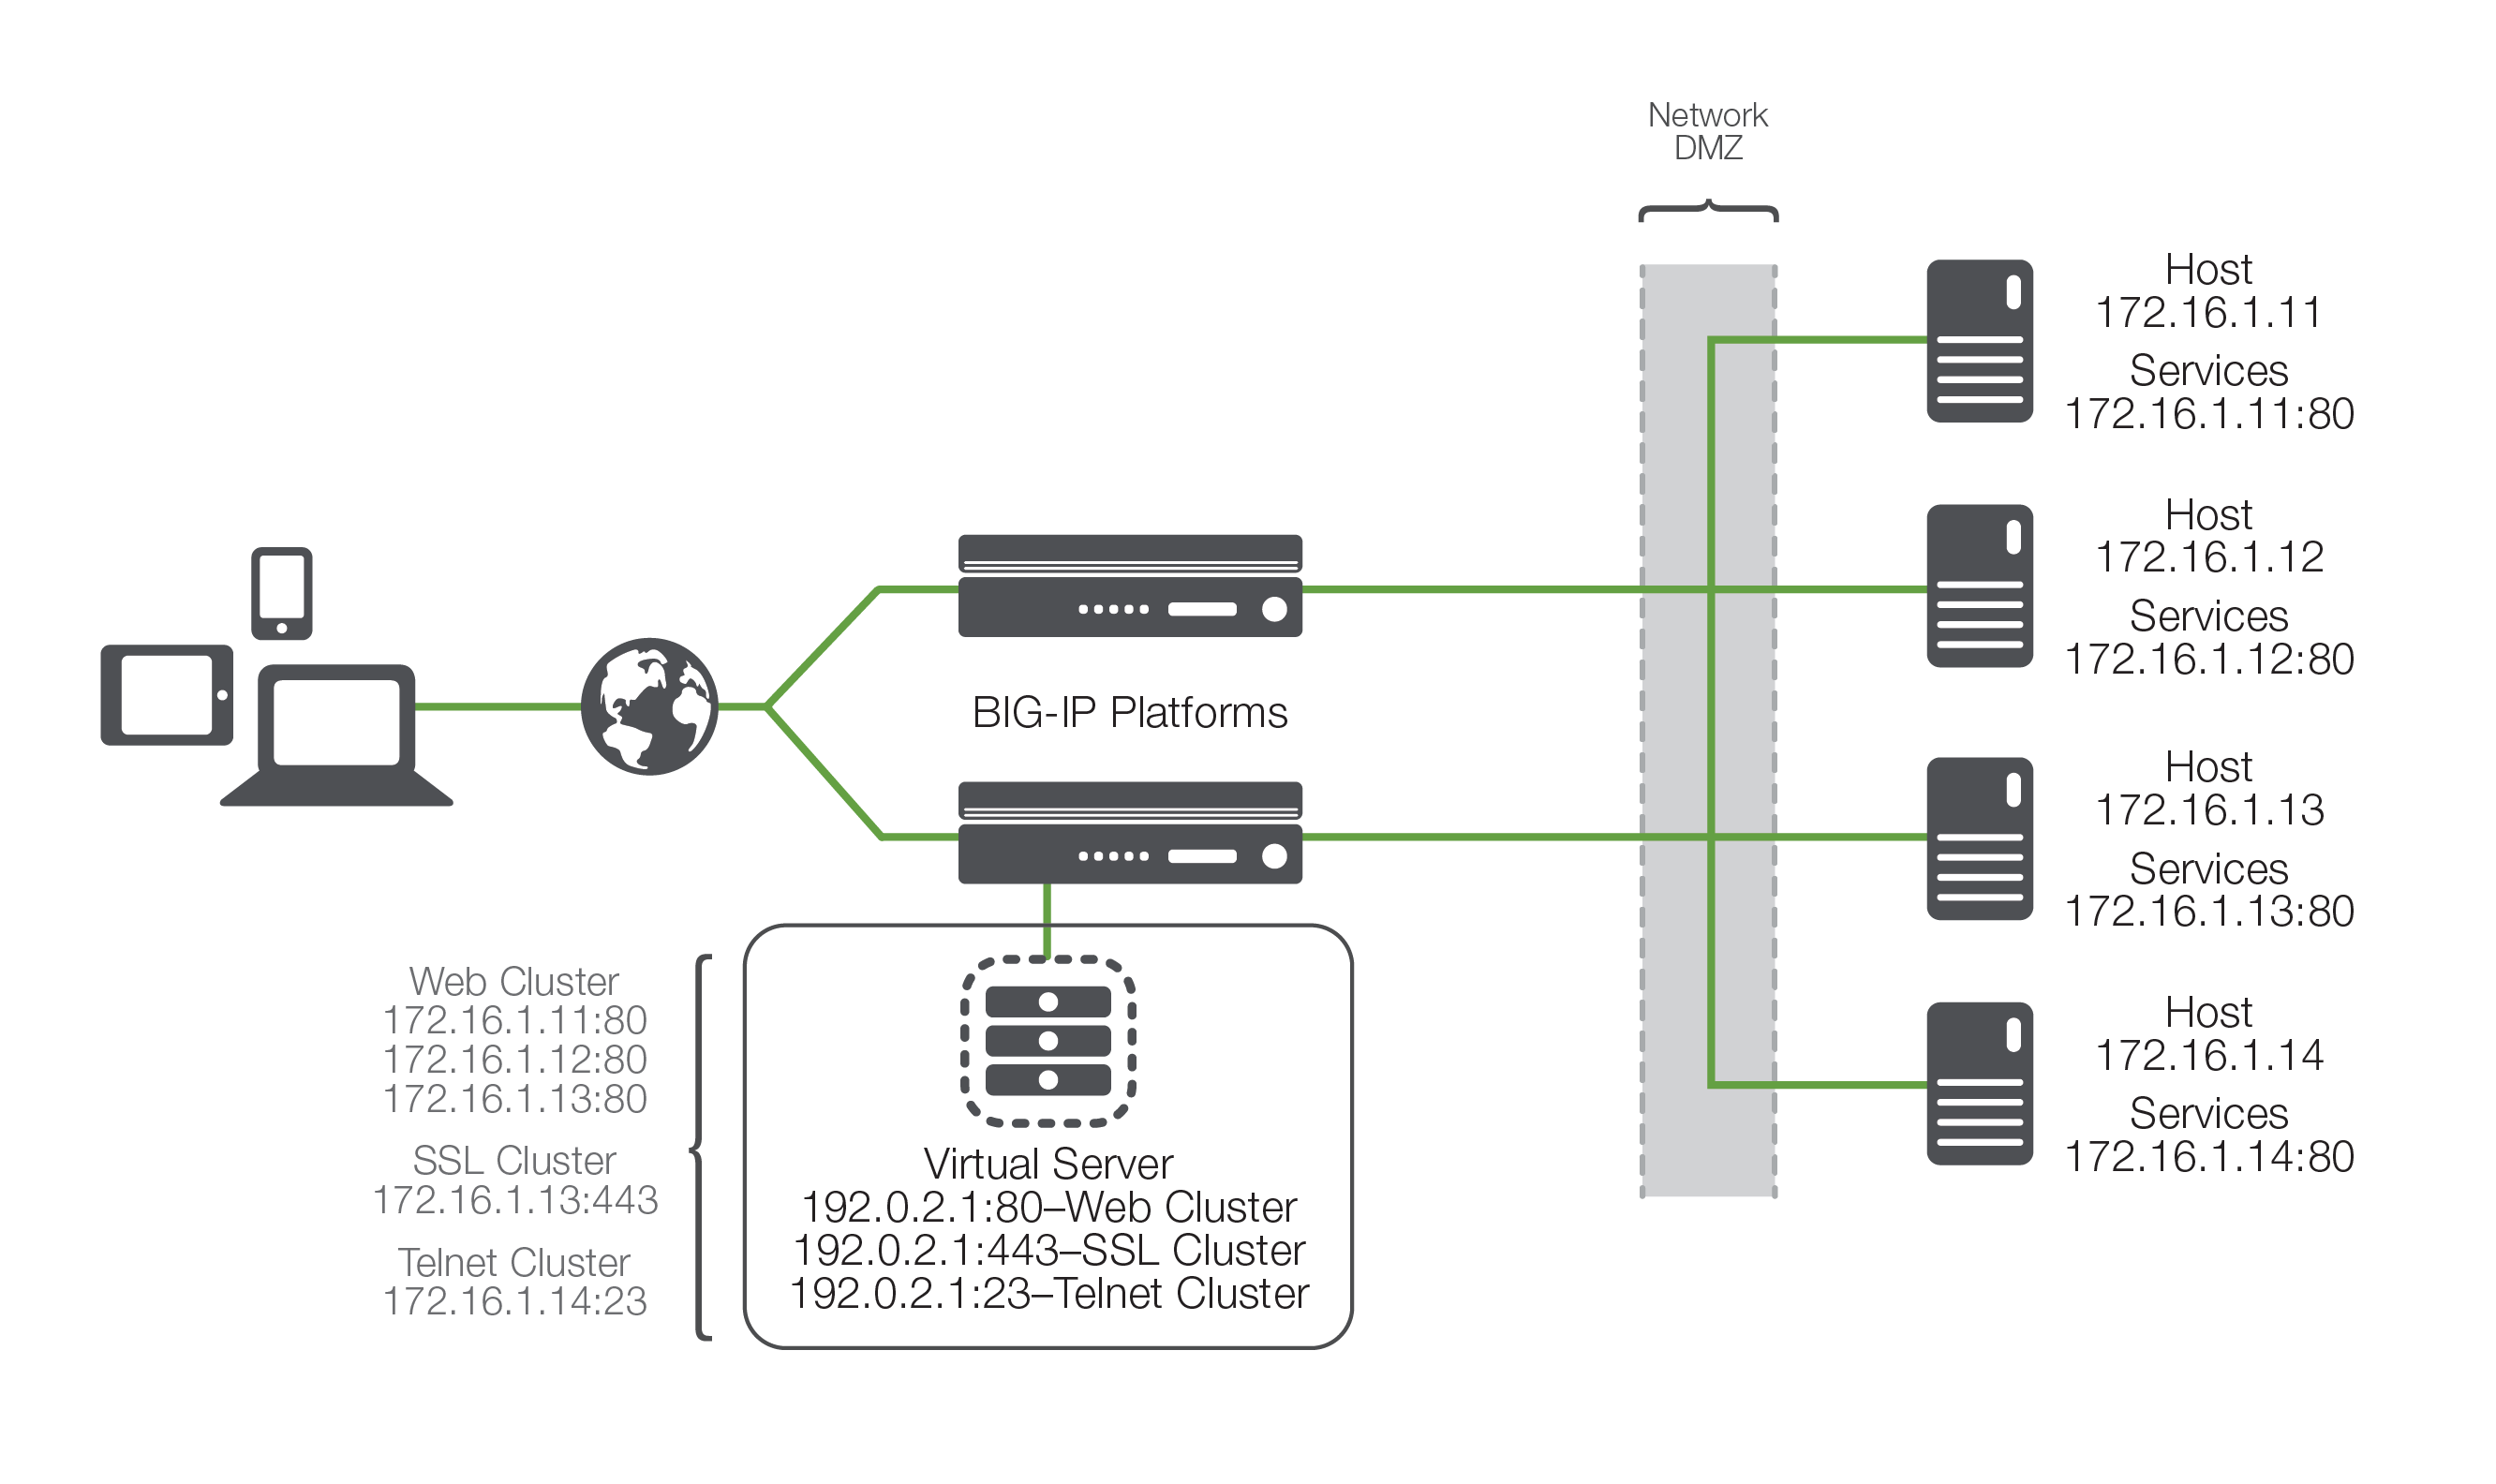
\includegraphics[width=\linewidth]{figures/nutbolt.png}
  \caption{High performance load balancing architecture~\cite{nutbolt}.}
\label{fig:nutbolt}
\end{figure}

\begin{figure}
  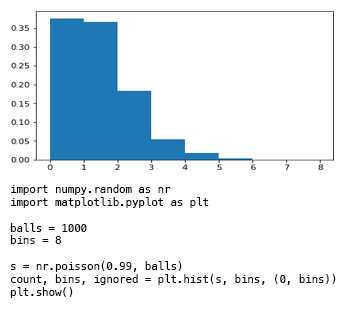
\includegraphics[width=\linewidth]{figures/poisson.png}
  \caption{What a Poisson distribution looks like}
\label{fig:poisson}
\end{figure}

\section{Project Description}
There are a number of load balancing algorithms that have been shown
to increase the overall performance of webservers when used in place
of random or RR, yet few are ever implemented in prevailing open
source projects. The biggest advantage of using RR and random from a
developers point of view is that they are intuitive algorithms that
are easy to implement and maintain. While dedicated hardware load
balancers continually take advantage of recent
innovation~\cite{nutbolt}, the open source community has been
continually left behind. My research is an attempt to bring some of
the most recent and successful load balancing techniques into
NGINX,~\footnote{\url{https://nginx.org}} the leading open source load
balancer and webserver.

Of these innovations, the algorithm in particular that I want to focus
on originally comes from Michael Mitzenmacher's 2001 paper,
\textit{The Power of Two Choices in Randomized Load
  Balancing}~\cite{mitzenmacher}. In this paper, Mitzenmacher outlines
an algorithm called two-choices, which behaves exponentially superior
to the traditional strategies like RR and random.
Figure~\ref{fig:supermarket} illustrates the two-choices algorithm in
what Mitzenmacher presents as the ``supermarket model'', where a
customer wishes to enter the least busy checkout queue. The idea
behind two-choices is that the efficient shopper only surveys two of
the available queues and quickly enters the least crowded one. The
less efficient shopper painstakingly compares every queue before
making a decision. Mitzenmacher found that by selecting two random
queues, it was possible to avoid the notorious ``thundering herd''
problem. If every customer was seeking the least crowded queue, then
at any given time, everyone will be racing towards a single lane,
largely ignoring everything else. Once that queue fills up, another
one is chased down. With two-choices, multiple customers are not
likely to be directed to the same queue, but they are very likely to
avoid the most crowded one.

\begin{figure}
  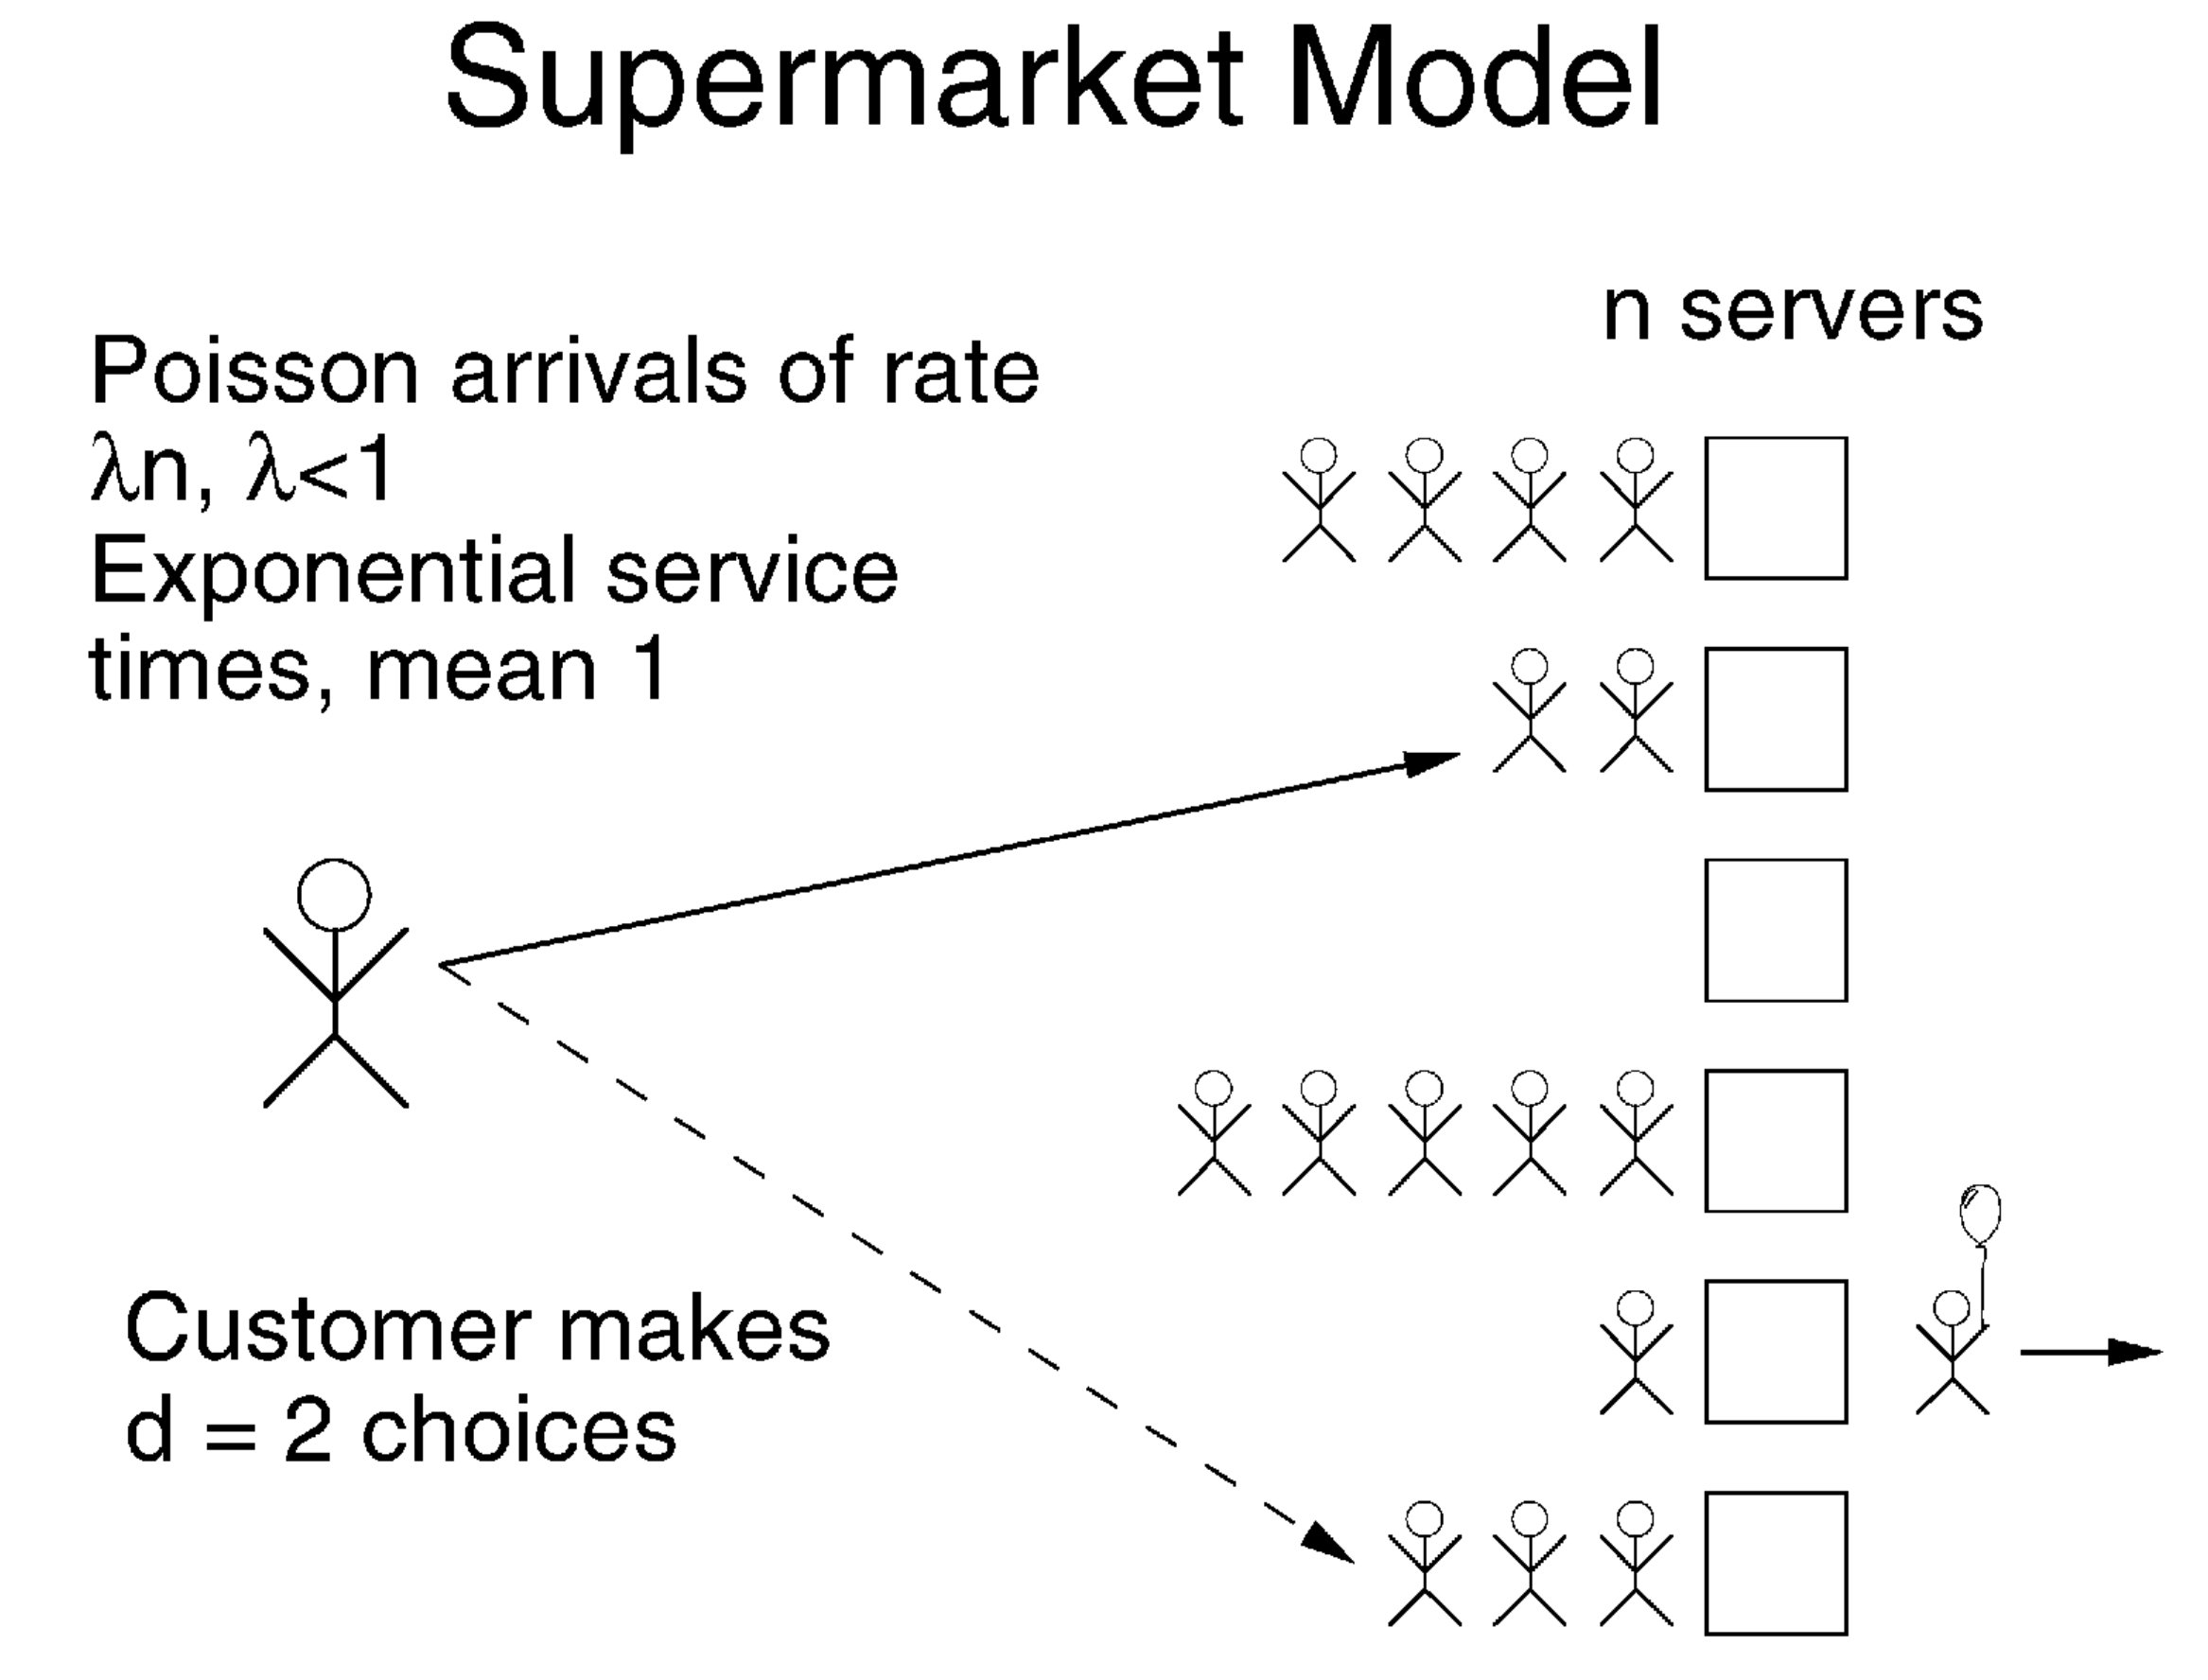
\includegraphics[width=\linewidth]{figures/supermarket.png}
  \caption{The two-choices load balancing algorithm as described in Mitzenmacher's paper.}
\label{fig:supermarket}
\end{figure}

The aim of my research project is to study the behavior of these
breakthrough load balancing techniques in a production environment. To
accomplish this I have two goals: (1) Reproduce the work of
Mitzenmacher and others relating to the efficiency of various load
balancing strategies. (2) Implement two-choices as an NGINX module and
test it against the other available load balancers.

\section{Experimental Setup}
This project was initially inspired by a talk given by Tyler McMullen,
titled \textit{Load Balancing is Impossible}~\cite{mcmullen}, where he
outlines the challenges load balancers face when dealing with the web
as we know it today. I began my research by expanding the initial
simulations given in his talk and soon I was able to construct an
environment where I could reproduce the work presented in research
papers regarding the two-choices algorithm.

I conducted my load balancing experimentation using an IPython
notebook~\cite{ipython} running inside a python virtual environment
because it enables portable and cross platform development. Using a
Poisson stream with a mean of 0.99 as my request distribution model, I
assigned a weight to each request to represent its arrival on the
server. In the IPython notebook I model the load balancing in the
following way: There is a list of length $n$ representing the requests
and a list of length $m$ representing the available servers. The
requests are passed to a load balancing algorithm which increments a
counter belonging to a particular server by that request's weight.
After all requests are distributed, the standard deviation of requests
among each server is compared between algorithms. A perfect load
distribution would therefore have a standard deviation of zero.

The algorithms I implemented were \emph{random}, \emph{round-robin},
and \emph{two-choices}: Random chooses a server for each request
independently and uniformly at random, RR distributes the request to
each server one by one, and two-choices first selects two servers
independently and uniformly at random and then chooses the server with
the least load to process the request. Figure~\ref{fig:notebook}
provides minimal algorithm implementations used in my initial testing
environment and gives a better sense of how my IPython simulation was
organized.

The later stages of my research was done using special configuration
files that allow my load balancing module to be dynamically linked to
the system installation of NGINX.\ In addition, I utilized the Go
programming language~\footnote{\url{https://golang.org/}} to build a
webserver which compiles into a native binary for execution on
multiple machines and ports. All of the software components used in my
research are provided within a single organized git
repository.~\footnote{\url{https://github.com/anschwa/capstone}}

\begin{figure}
  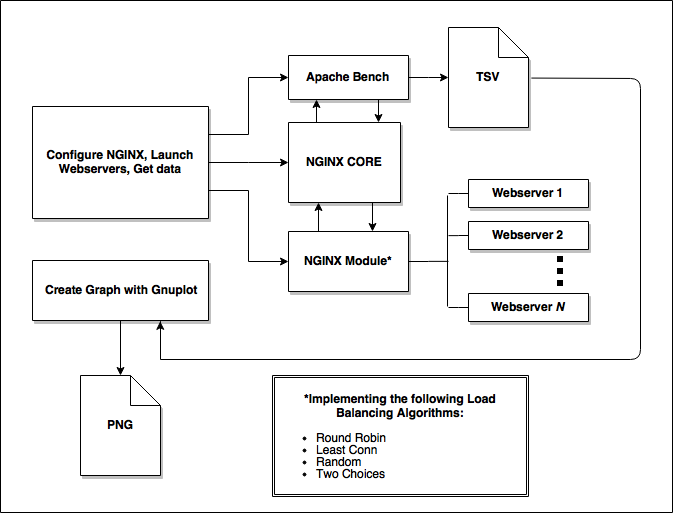
\includegraphics[width=\linewidth]{figures/software.png}
  \caption{Software architecture for running simulations with NGINX.}
\label{fig:software}
\end{figure}

\begin{figure}
\begin{verbatim}
import numpy as np
import numpy.random as nr

rate = nr.poisson(0.99, requests)
DIST = [(w * 0.1) + 1 for w in rate]

def uniform_random(requests, servers):
    rand = nr.randint(low=0, high=servers, size=requests)
    load = [0] * servers
    for i in range(requests):
        weight = DIST[i]
        chosen_server = rand[i]
        load[chosen_server] += weight
    return np.std(load)

def round_robin(requests, servers):
    load = [0] * servers
    for i in range(requests):
        weight = DIST[i]
        chosen_server = i % servers
        load[chosen_server] += weight
    return np.std(load)

def two_choices(requests, servers):
    load = [0] * servers
    for i in range(requests):
        choice_one = nr.randint(0, servers)
        choice_two = nr.randint(0, servers)
        
        if load[choice_one] < load[choice_two]:
            best_choice = choice_one
        else:
            best_choice = choice_two  

        weight = DIST[i]
        load[best_choice] += weight
    return np.std(load)
\end{verbatim}
\caption{Simplified Python Implementations}
\label{fig:notebook}
\end{figure}

\subsection{NGINX Module Development}
I developed two load balancing modules for NGINX:\ random and
two-choices. The underlying load balancer for NGINX is RR, but it also
provides a module called \emph{least_conn}, which will distribute
requests giving preference to the server with the least connections
currently established. The two-choices module is implemented by
incorporating the functionality provided by least_conn and my new
random module. Both modules are compiled and dynamically linked into
the system installation of NGINX because it makes development much
easier. However, both modules can can be statically linked if desired.
Although NGINX provides an API for writing modules in perl, I chose to
implement them directly in C to eliminate any potential overhead that
may skew the results. I also consider native NGINX module
implementations more useful to the open source community.

In order to test the effectiveness of the load balancing algorithms, I
created a simple webapp in Go that will simulate my production
webserver environment. Go is an excellent language to use for this
task because it has an extensive HTTP package in the standard library,
compiles to native machine code, and does not need any additional
dependencies to host a webserver.

The Go webapp generates a Poisson random number for each incoming
request. This number is then used to determine how long the webapp
will sleep for before sending back a response. I do this to simulate
the unpredictability of request duration and load on the server. I
chose to model my webserver environment with the Poisson process
because it is well understood and commonly used to model the behavior
of internet traffic. Naturally, this will not provide an accurate
model for all production web applications, however, I have produced a
workflow for benchmarking the performance of all NGINX load balancers,
including two-choices, on any given system. This workflow will allow
anyone to observe the performance of each algorithm in their own
production environments. Figure~\ref{fig:software} depicts the entire
benchmarking workflow and the general software architecture of this
project.

\subsection{Apache Bench Testing Strategy}
The industry standard tool for benchmarking and measuring web server
performance is a command line utility called Apache
Bench,~\footnote{\url{https://httpd.apache.org/docs/2.4/programs/ab.html}}
or \emph{ab}. The interface is quite simple, it allows you to specify
how many total requests to send to a website and how many should be
made concurrently. After sending the requests, \texttt{ab} will
provide some useful information such as the total time to complete the
requests, requests processed per second by the webserver, and the
average time spent per request. I use these metrics to gauge the
performance of the load balancers on NGINX in addition to graphing the
latency of each request in the benchmark.

\section{Results and Discussion}

\subsection{IPython Simulation Results}
My initial simulations reaffirmed the results presented by
Mitzenmacher. When requests are weighted, the standard deviation of
two-choices approaches zero as the amount of requests being processed
increases. As Figures~\ref{fig:python1} indicates, RR does much better
than random, but has an increasing standard deviation as requests
increase. Figure~\ref{fig:python3} highlights an important
observation: RR always completes in the least amount of time, whereas
two-choices takes more than twice as long to run. Also worth noting is
that when the number of servers are increased, RR performs more
similarly to two-choices, however, Figure~\ref{fig:python2} confirms
that two-choices is clearly better at maintaining a uniform
distribution of requests across all available servers. Although my
experiments reaffirms that two-choices is the superior algorithm as
far as load distribution, the results raise an important question: How
will the overhead of two-choices affect the latency of a production
webserver?

\begin{figure}
  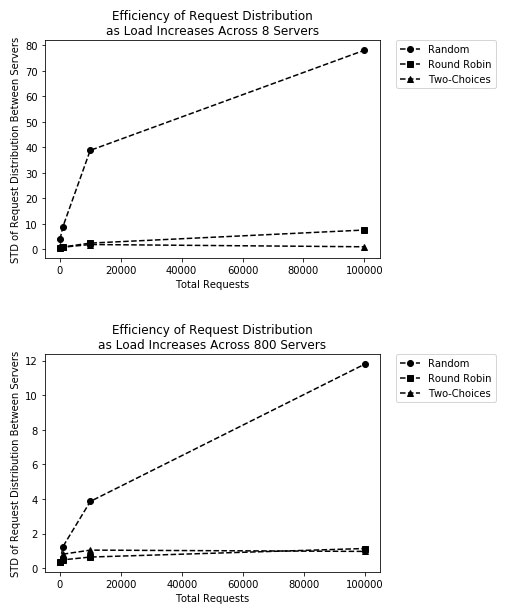
\includegraphics[width=\linewidth]{figures/py/all3.jpg}
  \caption{IPython notebook simulation results for random, round robin, and two-choices.}
\label{fig:python1}
\end{figure}

\begin{figure}
  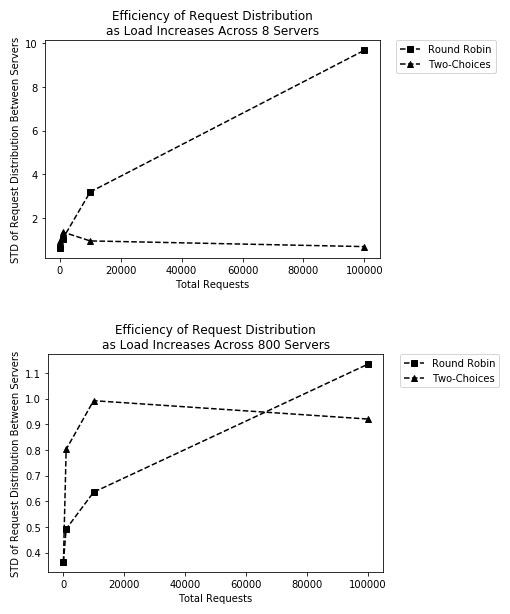
\includegraphics[width=\linewidth]{figures/py/all2.jpg}
  \caption{A closer look at the load distribution capabilities of round robin and two-choices.}
\label{fig:python2}
\end{figure}

\begin{figure}
\begin{verbatim}
8 Servers:
  Random: 410 ms ± 79 ms per loop
  Round Robin: 371 ms ± 18.5 ms per loop
  Two Choices: 826 ms ± 171 ms per loop
800 Servers:
  Random: 414 ms ± 53.9 ms per loop
  Round Robin: 381 ms ± 24.5 ms per loop
  Two Choices: 784 ms ± 9.04 ms per loop
\end{verbatim}
\caption{Latency of random, round robin, and two-choices in IPython
  simulation using the \texttt{timeit} module with 
  format: (mean ± std.\ dev.\ of 7 runs, 1 loop each).}
\label{fig:python3}
\end{figure}

\newpage\null\newpage
\subsection{NGINX Simulation Results}
My extensive benchmarking revealed no obvious distinction between load
balancing algorithms running in NGINX.\ Regardless of the active
module, performance remained about the same. However, there were some
general trends regarding concurrent and total requests that were
anticipated, namely, when you flood your webserver with requests, it
takes longer to respond.

What these results do indicate, is that the overhead of a load
balancer may become negligible when taking into account the total
overhead associated with completing an HTTP request. In the earlier
simulations with python, I was concerned that the increased latency of
two-choices would make it an inconvenient load balancer in a
production environment. However, my results show that we may be able
to take advantage of two-choice's uniform load distribution abilities
without paying much performance penalty.

Yet, the lack of a clear distinction in algorithms is a concern. It is
a good indication that my experimental environment is not capable of
simulating the conditions necessary to make high performance load
balancing observable. I'm not completely dismayed because using
\texttt{ab} to benchmark webserver performance is an industry
standard. Although, employing a custom benchmarking technique for
these experiments may have produced more obvious results. With that
being said, I'm still confident in the viability of two-choices as a
load balancer after running these experiments.

Additionally, the machine running all simulations can only launch up to 8
webservers, each processing up to 100 concurrent connections from
\texttt{ab}.~\footnote{Macbook Pro: Intel(R) Core(TM) i5-4288U CPU @
  2.60GHz, 16 GB 1600 MHz DDR3.} While it is possible that the load
balancing modules need to be tested with an NGINX configuration
containing hundreds of servers, it may be an unrealistic expectation.
When I initially contacted the NGINX mailing list about my research
project, lead developer Maxim Dounin responded that algorithms like
two-choices have never been considered for implementation because it
was unlikely to effect performance unless one was using NGINX in a
very large computing environment.
\footnote{``As far as I understand, \emph{power of two choices} might
  be beneficial if you need to optimize time spent on comparing the
  load on different balanced servers, for example, when balancing very
  large number of servers. Or when trying to do distributed balancing
  with multiple load balancers, and query loads directly from balanced
  servers.'' (2017-09-27)}

\begin{figure}
  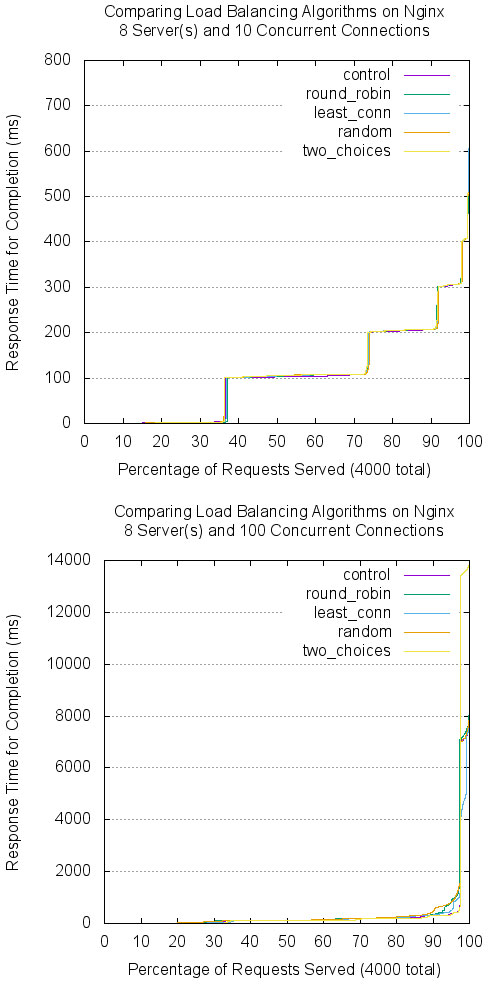
\includegraphics[width=\linewidth]{figures/ab/nginx/nginx-8.jpg}
  \caption{Each load balancing algorithm has near identical
    performance in NGINX according to the \textit{ab} results.}
\label{fig:nginx1}
\end{figure}

Most of my findings are summarized by Figure~\ref{fig:nginx1}. When
the number of concurrent connections are kept relatively low, each
load balancing module behaves nearly identical. However, as we
increase the concurrent connections, we see that the vast majority of
requests are completed under 500 ms, but approximately 5\% of requests
take thousands of milliseconds longer to complete. This behavior is a
known issue with using Apache Bench, but it also addresses the problem
load balancing attempts to solve. That is, once a webserver becomes
overloaded, it is very hard for it to recover.

The stair-step pattern represented in these graphs unsurprisingly
correspond directly with my Poisson distribution. Each incoming
request will spend either 0, 100, 200, or 300 ms on the webserver
before getting a response. The fact that we can visualize the Poisson
stream almost exactly is another indication that the overhead of load
balancing is negligible under these testing conditions and NGINX.\

In order to get a better sense of these seemingly homogeneous results,
I constructed another visualization for examining the minimum,
maximum, and average request latencies of each algorithm. It is
possible to observe some additional trends using these new charts.
Figure~\ref{fig:nginx2} reaffirms that under lower concurrency levels,
performance is pretty uniform between algorithms. However, it remains
unclear if any algorithm is superior under high levels of concurrency.
While it appears two-choices may occasionally have an advantage,
Figure~\ref{fig:nginx8} serves as a reminder how a few latency
outliers from Apache Bench can skew the graphs significantly.

Figure~\ref{fig:ab-stats} gives a more complete overview of the
\texttt{ab} benchmarking results from the simulations. While it is
certainly true that higher concurrency levels increase the overall
latency of the NGINX server, the median and mean latencies are not
heavily effected.

\begin{figure}
  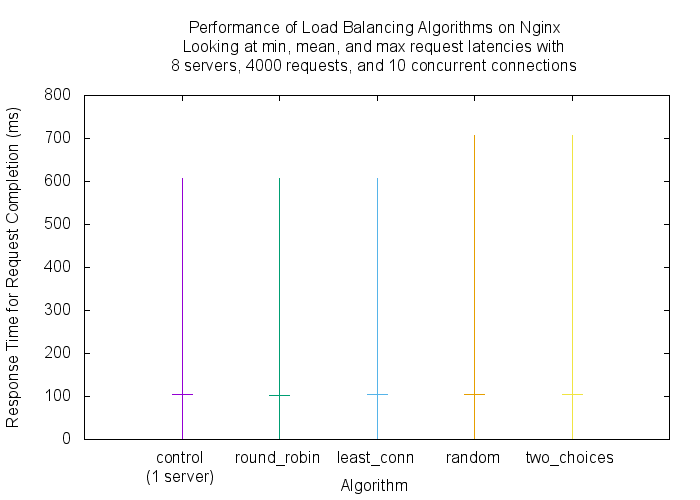
\includegraphics[width=\linewidth]{figures/ab/stats/10/stats-8.png}
  \caption{Under low levels of concurrency, there are less outliers
    so it's possible to see the slight variations in performance.}
\label{fig:nginx2}
\end{figure}

\begin{figure}
  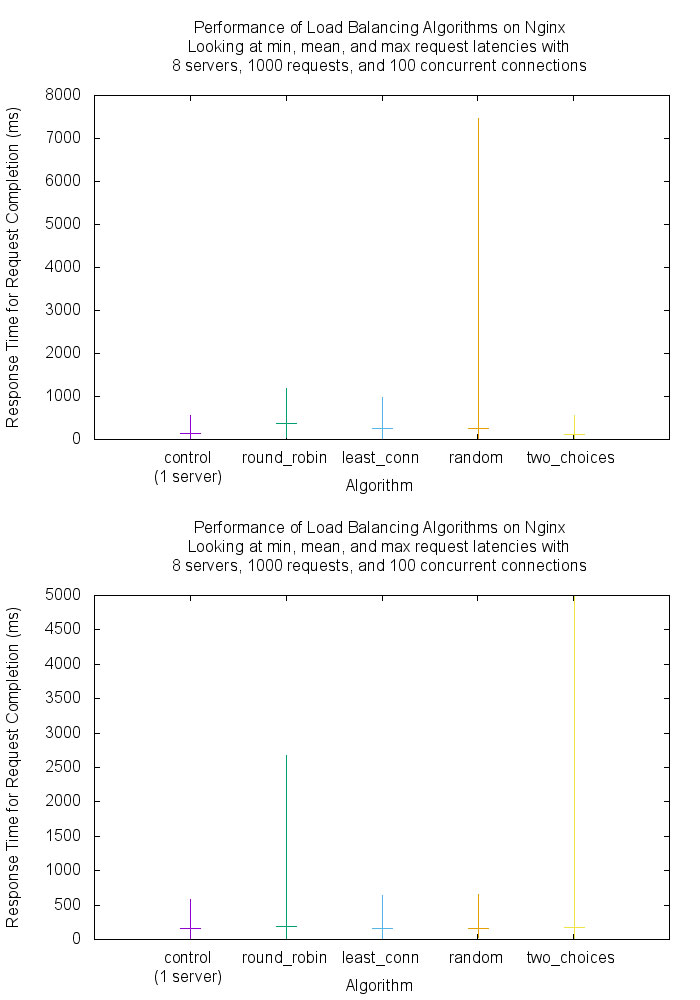
\includegraphics[width=\linewidth]{figures/ab/stats/100/stats-8.jpg}
  \caption{Although \texttt{ab} is a great benchmarking tool, results
    are often inconsistent due to a few outliers.}
\label{fig:nginx8}
\end{figure}

\begin{figure}
\centering
\resizebox{\columnwidth}{!}{%
\begin{tabular}{l c c c c c r}
algorithm & concurrency & min & mean & [+/-sd] & median & max \\
\hline
control     & 10 & 1 & 107 & 123.6 & 103 & 1351 \\
round_robin & 10 & 1 & 106 & 102.5 & 105 & 607 \\
least_conn  & 10 & 0 & 103 & 102.4 & 105 & 605 \\
random      & 10 & 1 & 106 & 103.8 & 104 & 707 \\
two_choices & 10 & 0 & 101 & 100.6 & 104 & 603 \\
\\
control     & 50 & 1 & 108 & 103.0 & 103 & 613 \\
round_robin & 50 & 1 & 245 & 742.1 & 111 & 7187 \\
least_conn  & 50 & 1 & 109 & 185.2 & 104 & 7100 \\
random      & 50 & 1 & 187 & 321.4 & 118 & 3047 \\
two_choices & 50 & 1 & 146 & 257.6 & 106 & 4473 \\
\\
control     & 100 & 1 & 164 & 205.1 & 118 & 3186 \\
round_robin & 100 & 1 & 194 & 559.5 & 108 & 14004 \\
least_conn  & 100 & 1 & 177 & 416.8 & 119 & 11747 \\
random      & 100 & 1 & 212 & 559.0 & 132 & 13673 \\
two_choices & 100 & 1 & 187 & 334.4 & 115 & 3340 \\
\end{tabular}
}
\caption{Raw \texttt{ab} statistics for 8 Servers and 4,000 total requests}
\label{fig:ab-stats}
\end{figure}

\section{Related And Future Work}
Overall, I'm excited by the outcomes of my capstone research project.
If I continue running experiments on more sophisticated server
environments I hope to get a more refined result set that will lead to
a better understanding of NGINX load balancing performance. I plan to
contribute my two-choices module upstream to the NGINX project as well
as respond to any feedback I may get from the other open source
developers. Additionally, it would be worthwhile to gather more data
and research production web application server load more thoroughly.
The Poisson distribution is a great statistical model for a
proof-of-concept, but my research would definitely benefit from a
richer statistical dataset. Load balancing for the most part is
primarily a concern for large companies and data centers. For this
reason, much of my background research involved learning how the big
tech companies are approaching this problem. The prevailing strategies
to the load balancing problem usually involves optimization deeper
within the networking stack, where the problem can be more discretely
defined and more generally applied.

\subsection{Microsoft's JIQ}
Join-Idle-Queue is the latest and greatest load balancing algorithm.
It was developed by Microsoft and achieves greater performance than
two-choices and another competing algorithm called
join-shortest-queue. However, JIQ does not introduce communication
overhead on the servers. This is achieved by only using local
information about server load. The idea behind JIQ is to ``decouple
discovery of lightly loaded servers from job assignment''~\cite{jiq}.
This is achieved through utilizing idle CPUs to make the load
balancing decision. JIQ out-performs the competing advanced load
balancing algorithms and much like my results, Microsoft notes that
these load balancing strategies are most noticeable under extremely
high server load.

\subsection{Google's BBR}
BBR stands for Bottleneck Bandwidth and Round-trip propagation time.
It is a new congestion control algorithm developed and deployed by
Google for increasing the throughput of TCP~\cite{bbr}. The purpose of
the algorithm is to measure the current bottleneck of the network and
only send enough data to ``fill the pipe''. The success of the
algorithm comes from measuring network congestion in terms of its
bottleneck instead of packet loss, which is how it is traditionally
done. Additionally, it was found that maximum throughput is achieved when
the loss rate was less than the inverse square of the bandwidth delay
product (BDP). BBR is already implemented in the Linux kernel for
TCP.\

\subsection{Facebook's Egress}
Egress is a process for evaluating network latency and congestion
through ``performance aware routing'' on Facebook’s
network~\cite{egress}. The Egress paper explains some key elements of
running a network on a massive scale that minimizes congestion. What
Google did with TCP congestion, Facebook did with the border gateway
protocol (BGP); they made it ``capacity and performance aware''.
Essentially, Facebook had to optimize its point of presence (PoP)
servers to have highly efficient routing algorithms by establishing
shorter paths, to deliver content to its billions of users. This paper
illustrates a common theme that traditional implementations of
networking protocols are no longer sufficient.

\subsection{Linux Socket Balancing: Epoll-and-Accept}
An interesting problem about NGINX was discussed by Marek Majkowski of
CloudFlare, where he examines how Linux schedules connections to
sockets~\cite{epoll}. NGINX, like many applications may create
multiple worker processes to increase performance at scale. On Linux,
these processes communicate over sockets. On NGINX, a single socket
``listens'' for new connections and then distributes them to one of
the available worker processes. This behavior is exactly like the load
balancing discussed in this paper, except that instead of processing a
request on another webserver, at this level, NGINX distributes new
connections among OS processes. It is also possible to have a model
where there are multiple listening sockets and multiple worker
processors. Unfortunately for Linux, when distributing connections
between sockets using \texttt{epoll()} to avoid blocking on the
\texttt{accept()} system call, the scheduling behavior becomes
Last-In-First-Out (LIFO).\ That is, the busiest process will be
selected most often. Just like the thundering herd problem, this
results in an unbalanced worker process load and a decrease in NGINX
performance. However, by setting the \texttt{SO_REUSEPORT} socket
option, each worker process will have a more uniform load at the cost
of higher latency.

\section{Acknowledgments}
I want to give a special thanks to David Barbella for being my
Capstone Adviser and Charlie Peck for offering additional guidance
during my project. I would also like to thank Maxim Dounin for
answering my questions on the NGINX mailing list.


\bibliographystyle{ACM-Reference-Format}
\bibliography{sources} 

\end{document}
